\makeatletter\def\input@path{{minimus}{standalone-silicon}}\makeatother

\documentclass{standalone-silicon}

\usepackage{minimus-text}
\usepackage{minimus-math}
\usepackage{minimus-tikz}

\begin{document}
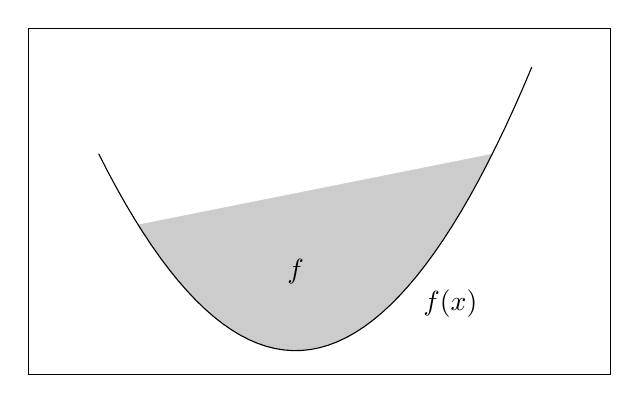
\begin{tikzpicture}

\def\func#1{0.4*#1*#1}

\fill[black!20!white] plot[domain=-2.0:2.5,samples=50] (\x,{\func{\x}}) -- cycle ;
\draw plot[domain=-2.5:3,samples=50] (\x,{\func{\x}}) ;
\path (1.5,\func{1.5}) node[below right] (Func) {$f(x)$} ;
\path (0,1) node[] (Epi) {$\epi f$} ;  

\path (-3.4,-0.3) coordinate (SW) ; 
\path (+4.0,4.1) coordinate (NE) ; 

\draw[ultra thin] (SW) rectangle (NE) ;

\end{tikzpicture}
\end{document}